%%%%%%%%%%%%%%%%%%% vorlage.tex %%%%%%%%%%%%%%%%%%%%%%%%%%%%%
%
% LaTeX-Vorlage zur Erstellung von Projekt-Dokumentationen
% im Fachbereich Informatik der Hochschule Trier
%
% Basis: Vorlage svmono des Springer Verlags
%
%%%%%%%%%%%%%%%%%%%%%%%%%%%%%%%%%%%%%%%%%%%%%%%%%%%%%%%%%%%%%

\documentclass[envcountsame,envcountchap, deutsch]{i-studis}

\usepackage{makeidx}         	% Index
\usepackage{multicol}        	% Zweispaltiger Index
%\usepackage[bottom]{footmisc}	% Erzeugung von Fu�noten

%%-----------------------------------------------------
%\newif\ifpdf
%\ifx\pdfoutput\undefined
%\pdffalse
%\else
%\pdfoutput=1
%\pdftrue
%\fi
%%--------------------------------------------------------
%\ifpdf
\usepackage[pdftex]{graphicx}
\usepackage{epstopdf}
\usepackage[pdftex,plainpages=false]{hyperref}
%\else
%\usepackage{graphicx}
%\usepackage[plainpages=false]{hyperref}
%\fi

%%-----------------------------------------------------
\usepackage{color}				% Farbverwaltung
%\usepackage{ngerman} 			% Neue deutsche Rechtsschreibung
\usepackage[english, ngerman]{babel}
%\usepackage[latin1]{inputenc} 	% Erm�glicht Umlaute-Darstellung
\usepackage[utf8]{inputenc}  	% Erm�glicht Umlaute-Darstellung unter Linux (je nach verwendetem Format)

%-----------------------------------------------------
\usepackage{listings} 			% Code-Darstellung
\lstset
{
	basicstyle=\scriptsize, 	% print whole listing small
	keywordstyle=\color{blue}\bfseries,
								% underlined bold black keywords
	identifierstyle=, 			% nothing happens
	commentstyle=\color{red}, 	% white comments
	stringstyle=\ttfamily, 		% typewriter type for strings
	showstringspaces=false, 	% no special string spaces
	framexleftmargin=7mm, 
	tabsize=3,
	showtabs=false,
	frame=single, 
	rulesepcolor=\color{blue},
	numbers=left,
	linewidth=146mm,
	xleftmargin=8mm
}
\usepackage{textcomp} 			% Celsius-Darstellung
\usepackage{amssymb,amsfonts,amstext,amsmath}	% Mathematische Symbole
\usepackage[german, ruled, vlined]{algorithm2e}
\usepackage[a4paper]{geometry} % Andere Formatierung
\usepackage{bibgerm}
\usepackage{array}
\usepackage{caption}
\hyphenation{Ele-men-tar-ob-jek-te  ab-ge-tas-tet Aus-wer-tung House-holder-Matrix Le-ast-Squa-res-Al-go-ri-th-men} 		% Weitere Silbentrennung bei Bedarf angeben
\setlength{\textheight}{1.1\textheight}
\pagestyle{myheadings} 			% Erzeugt selbstdefinierte Kopfzeile
\makeindex 						% Index-Erstellung


%--------------------------------------------------------------------------
\begin{document}
%------------------------- Titelblatt -------------------------------------
\title{Titel der Arbeit auf Deutsch}
\subtitle{English Title}
%---- Die Art der Dokumentation kann hier ausgew�hlt werden---------------
%\project{Bachelor-Projektarbeit}
%\project{Bachelor-Abschlussarbeit}
%\project{Master-Projektstudium}
\project{Master-Abschlussarbeit}
%\project{Seminar zur Vorlesung ...}
%\project{Hausarbeit zur Vorlesung ...}
%--------------------------------------------------------------------------
\supervisor{Titel Vorname Name} 		% Betreuer der Arbeit
\author{Bachvarov, Vladislav} 							% Autor der Arbeit
\address{Ort,} 							% Im Zusammenhang mit dem Datum wird hinter dem Ort ein Komma angegeben
\submitdate{Abgabedatum} 				% Abgabedatum
%\begingroup
%  \renewcommand{\thepage}{title}
%  \mytitlepage
%  \newpage
%\endgroup
\begingroup
  \renewcommand{\thepage}{Titel}
  \mytitlepage
  \newpage
\endgroup
%--------------------------------------------------------------------------
\frontmatter 
%--------------------------------------------------------------------------
\preface

Ein Vorwort ist nicht unbedingt n�tig. Falls Sie ein Vorwort schreiben, so ist dies der Platz, um z.B. die Firma vorzustellen, in der diese Arbeit entstanden ist, oder einigen Leuten zu danken, die in irgendeiner Form positiv zur Entstehung dieser Arbeit beigetragen haben. Auf keinen Fall sollten Sie im Vorwort die Aufgabenstellung n�her erl�utern oder vertieft auf technische Sachverhalte eingehen.				% Vorwort (optional)


\kurzfassung
\inputencoding{latin1}
\paragraph*{}

Diese Arbeit befasst sich mit dem Thema Natural-Language-Processing (NLP), pr�ziser gesagt Transformer. In den ersten Kapiteln der Arbeit wird eine Einf�hrung in das Thema Vektorrepr�sentation von W�rtern gegeben. Nachfolgend werden die Modelle Transformer und BERT erkl�rt und schlie�lich wird die Struktur als Programmcode dargestellt. Das letzte und wichtigste Kapitel verschafft einen �berblick �ber Neural-Machine-Translation und die Anwendung solcher Modelle f�r die �bersetzung. Anschlie�end werden diese Modelle untersucht und eine Schlussfolgerung anhand der Ergebnisse wird gezogen.

%% deutsch
%\paragraph*{}
%In der Kurzfassung soll in kurzer und pr�gnanter Weise der wesentliche Inhalt der Arbeit beschrieben werden. Dazu z�hlen vor allem eine kurze Aufgabenbeschreibung, der L�sungsansatz sowie die wesentlichen Ergebnisse der Arbeit. Ein h�ufiger Fehler f�r die Kurzfassung ist, dass lediglich die Aufgabenbeschreibung (d.h. das Problem) in Kurzform vorgelegt wird. Die Kurzfassung soll aber die gesamte Arbeit widerspiegeln. Deshalb sind vor allem die erzielten Ergebnisse darzustellen. Die Kurzfassung soll etwa eine halbe bis ganze DIN-A4-Seite umfassen.
%
%Hinweis: Schreiben Sie die Kurzfassung am Ende der Arbeit, denn eventuell ist Ihnen beim Schreiben erst vollends klar geworden, was das Wesentliche der Arbeit ist bzw. welche Schwerpunkte Sie bei der Arbeit gesetzt haben. Andernfalls laufen Sie Gefahr, dass die Kurzfassung nicht zum Rest der Arbeit passt.

%% englisch
%\paragraph*{}
%The same in english.
 			% Kurzfassung Deutsch/English
\tableofcontents 						% Inhaltsverzeichnis
\listoffigures 							% Abbildungsverzeichnis (optional)
\listoftables 							% Tabellenverzeichnis (optional)
%--------------------------------------------------------------------------
\mainmatter                        		% Hauptteil (ab hier arab. Seitenzahlen)
%--------------------------------------------------------------------------
% Die Kapitel werden in separaten .tex-Dateien abgelegt und hier eingebunden.
\chapter{Einleitung und Problemstellung}

Begonnen werden soll mit einer Einleitung zum Thema, also Hintergrund und Ziel erl�utert werden.

Weiterhin wird das vorliegende Problem diskutiert: Was ist zu l�sen, warum ist es wichtig, dass man dieses Problem l�st und welche L�sungsans�tze gibt es bereits. Der Bezug auf vorhandene oder eben bisher fehlende L�sungen begr�ndet auch die Intention und Bedeutung dieser Arbeit. Dies k�nnen allgemeine Gesichtspunkte sein: Man liefert einen Beitrag f�r ein generelles Problem oder man hat eine spezielle Systemumgebung oder ein spezielles Produkt (z.B. in einem Unternehmen), woraus sich dieses noch zu l�sende Problem ergibt.

Im weiteren Verlauf wird die Problemstellung konkret dargestellt: Was ist spezifisch zu l�sen? Welche Randbedingungen sind gegeben und was ist die Zielsetzung? Letztere soll das
beschreiben, was man mit dieser Arbeit (mindestens) erreichen m�chte.
\chapter{Word2Vec}

In dieser Kapitel wird das Verfahren "Word2Vec" durch die Nutzung von Neuronalem Netz vorgestellt. Word2Vec ist eine Darstellung von Wörtern mit Vecoren, was auch aus die Abkürzung klar wird - Word ist klar; 2 - to; und Vec - Vector und das ganze "word to vector". Dieses Model ist am meisten  in der Natural Laguage Processing (NLP) verbreitet und wird in vielen Bereichen der Informatik genutzt, unter anderem in Spamfilterung und Dokumentenanalyse. Jedoch diese Technik besagt nur wie die Wörter eines Textes dargestellen werden können. Das Verfahren, bei dem die möglichst passenden Vektoren in einem ausgewählten Text, auch Corpus genant, gelernt werden, heißt Word Embeddings. Bei dieser Technik wird ein Neuronales Netzt eigesetzt. Die Vorgehensweise und die Idee wird folglich erklärt.

\section{Word Embedding}

Wie es schon in der Einleitung erwähnt wurde, Word Embedding ist der Prozess, bei dem die Wörter eines Textes in mathematischen Vektoren gewandelt werden. Zuerst muss der Corpus vorbeiretet werden. Ich stelle hier nur die Theorie und in einer späteren Kapitel (!? WICHTIG WELCHE GENAU!?) gehe ich tiefer in dem Programmcode.

\!!! DAS HIER GEHÖRT IN EINE ANDERE KAPITEL !!!
!!! DIE KAPITEL FÜR TEXTVORBEREITUNG ODER SOWAS!!!

Als der Text vorbeitet ist, sodass es von Sonderzeichen und alle unnötigen Zeichen bereinigt wird. Wenn der Text vorbeireitet ist, werden die Wörter aus dem Corpus bestimmt und jeder erhält einen Index. Üblicherweise werden die Wörter nach ihrer Häufigkeit angeordnet. Das häufigste Wort erhält somit den Index 1. Als nächstes werden die Wörter im Korpus durch ihren Index ersetzt, um alle Trainingspaare fürs Lernen generiert zu werden. Dies erfolgt in dem es durch das Corpus iteriert und in einem bestimmten Fenster, oder in der Literatur auch als Window gezeichnet, alle Contextwörter und den Targetwort ausgelesen werden. Das Targetwort ist das Wort in der Mitte, während die Wörter um das Targetwort entsprechend die Kontextwörter. 

!!! BIS HIER MUSS WEG !!!!

In der Literatur werden zwei Arten von Wort2Vec Modelle - SKIP-gram und CBOW (Continous Bag of Words). Beide Modelle verwenden ein Neuronales Netz mit einem oder zwei versteckten Schichten (siehe !!KAPITEL MIT DEM PROGRAMMCODE!!). Die beiden Methoden unterscheiden sich nach ihren Ein- und Ausgaben.   

\subsubsection{SKIP-gram Model}
Bei dem SKIP-gram-Model fließen die Targetwörter als Eingabe und das Model versucht ein Kontextwort zu raten. Hier ist die Struktur eines Skip-gram Models:

\begin{figure}
	\centering
	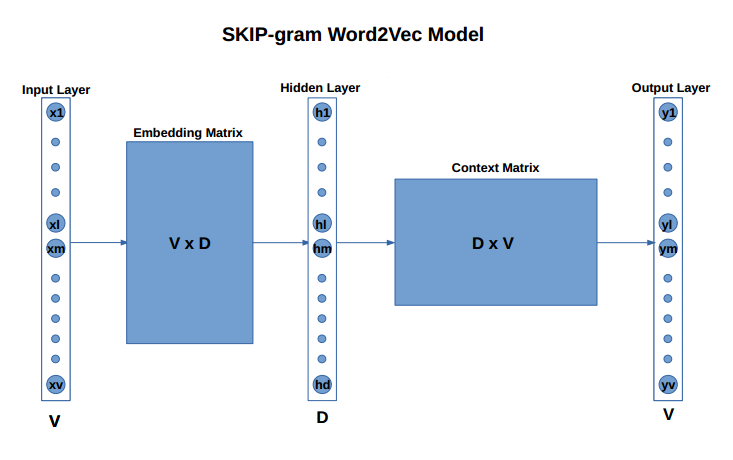
\includegraphics[scale=0.5]{images/SKIP_Model.png}
	\caption{Skip-gram Word2Vec Model}
	\label{skip}
\end{figure}

Aus der Abbildung \ref{skip} ist es zu entnehmen, dass ein Skip-gram Model aus einer hidden Schicht und zwei Eigabeschichten. Die Eingabe sowie die Ausgabe ist ein Vektor, der aus $\emph{V}$ Componente besteht. Das entspricht die größe des Wörterbuchs (engl. Vocabulary). Das versteckte Schicht besteht aus $\emph{D}$ Variablen und stellt einen Vektor dar. Die Dimensionalität dieses Vektors nimmt üblich einen Wert zwischen 25 und 300. Diese Variablen können auch als Eigenschaften für die Wörter betrachtet werden. Je mehr Kriterien es untersucht werden, desto besser die Beziehung zwischen Wörtern wiederspiegelt werden kann. Die Ausgabe ist wieder einen $\emph{V-dimensionalen}$ Vektor. Jedoch die Ausgabe ist kein One-Hot Vektor mehr, der das Kontextwort wiedergibt, sondern einen Wahrscheinlichkeitsvektor, dass der Wort mit der entsprechenden Index der richtige Contextwort ist.

Die zwei Matrizen sind identisch, jedoch die Kontextmatrize ist die transponierte Embeddingsmatrize. Diese Matrix beinhaltet unsere Wortvektoren.

Der Abbildung \ref{skip} nach besteht das neuronale Netz aus drei Schichten. Im Hiddenlayer steht ein Vektor, der abhängig von unsere Eingabe den Wortvektor repräsentiert. Die Ausgabe ist ein softmax

\subsubsection{CBOW Model}
Die Kontextwörter sind die Eingabe in dem CBOW-Model und das Model ratet der Targetwort. Die zwei Modelle besitzen die gleiche Anzahl an Schichten. Das CBOW-Model ist ein umgedrehtes SKIP-gram-Model, jedoch die Eingabe besteht aus $\emph{w}$-Viele Vektoren statt nur eins. Als nächstes stellt die \ref{cbow} Abbildung die beschriebene Struktur.

\begin{figure}
	\centering
	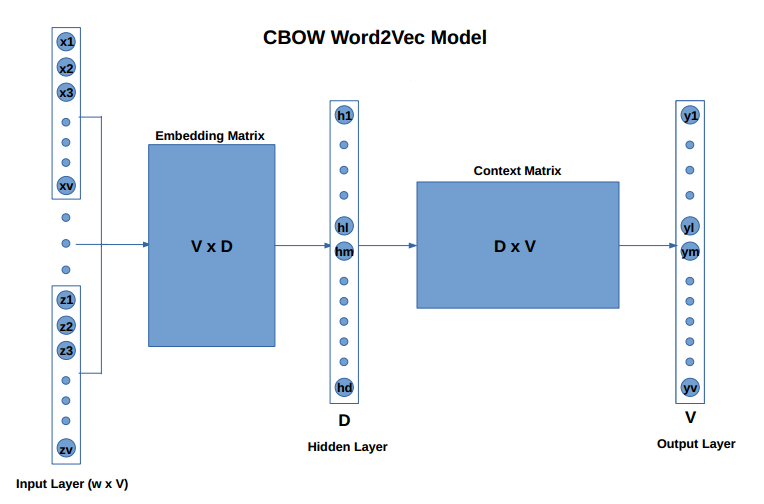
\includegraphics[scale=0.5]{images/CBOW_Model.png}
	\caption{CBOW Word2Vec Model}
	\label{cbow}
\end{figure}

Die Struktur des CBOW-Models besteht wieder aus eine Matrix für das Embedding der Target- und Kontextwörter. Die größe der Matrizen hängt von der ausgewählten Hyperparameter und die Größe des Datensatzes. Die Anzahl der verwendeten Inputvektoren entspricht die größe des gesetzten Window (Kontextfenster).

\subsection{Implementierung}
\chapter{GloVe}

Die Idee von \textbf{Glo}bal \textbf{Ve}ctors ist es, den Sinn hinter einem Wort in numerischer Vektorform darzustellen. GloVe ist eine weitere Möglichkeit neben word2vec(\cref{word2vec}) wie man Wörter oder sogar ganze Texte als Vektoren repräsentiert.

\section{GloVe-Methode}
Einige Variablen werden zuerst eingeleitet. Die Matrix der Word-Word-co-occu-rrence wird mit \textbf{$X$} notiert und eine beliebige Komponente in der Matrix mit \textbf{$X_{ij}$}. Der Wert \textbf{$X_{ij}$} stellt dar, wie oft das Wort \textit{j} in dem Kontext vom Wort \textit{i} vorkommt. Weiterhin beschreibt die Einheit \textbf{$X_i$} die Anzahl des Vorkommens eines beliebigen Wortes in dem Kontext vom Wort \textit{i} und ist in der folgenden \cref{x_i} definiert:

\begin{equation}
	X_i = \sum_{k} X_{ik}. \cite{GloVe:14}
	\label{x_i}
\end{equation}

Schließlich definieren wir die Einheit \textbf{$P_{ij}$}, die beschreibt, wie hoch die Wahrscheinlichkeit ist, dass ein Wort \textit{j} in dem Kontext vom Wort \textit{i} vorkommt. Die Formel ist in der \cref{p_ij} aufgeführt:

\begin{equation}
	P_{ij} = P(j|i) = \frac{X_{ij}}{X_i}. \cite{GloVe:14}
	\label{p_ij}
\end{equation}

Ein kleines Beispiel wird angegeben, damit verstanden werden kann, wie bestimmte Aspekte aus dem gemeinsamen Auftreten von Wörtern gewonnen werden können. Es werden zwei Wörter \textit{i} und \textit{j} betrachtet, die in einem Corpus vorkommen. Das Beispiel stammt aus dem Artikel \cite{GloVe:14} und ist aus dem Themenbereich des thermodynamischen Zustands. Nehmen wir die Wörter \textit{$i = ice$} und \textit{$j = steam$}. Die Beziehung der beiden Wörter kann so untersucht werden, indem die Relation mit anderen Probewörtern \textit{k} berechnet wird. Für Wörter, die in direktem Bezug zu \textit{$i = ice$} stehen, erwarten wir, dass das Verhältnis $\frac{P_{ik}}{P_{jk}}$ groß ist, zum Beispiel wenn das Wort \textit{$k = solid$} gewählt wird. Analoge Beziehung kann bei Wörtern betrachtet werden, die näher an Bedeutung zu \textit{$j = steam$} stehen. In solchen Fällen werden wir einen kleineren Wert des Bruchs $\frac{P_{ik}}{P_{jk}}$ erhalten - zum Beispiel wählen wir das Wort \textit{$k = gas$}. Selbstverständlich ist der Wert des Bruchs gleich eins, wenn das Wort \textit{k} zu beiden Wörtern \textit{i, j} in Korrelation steht, oder wenn sich keine Korrelation ergibt. Als Beispiel können wir das Wort \textit{$k = sun$} wählen. Die \cref{ice_steam_tab} stellt das Verhältnis zwischen den Wörtern dar:

	\begin{table}[]\label{tab_1}
		\centering
		\begin{tabular}{l|l|l|l|l}
			Probability and Ration & k = solid                                           & k = gas                                             & k = water                                           & k = fashion                                         \\ \hline
			P(k|ice)               & 1.9\times 10^{-4} & 6.6\times 10^{-5} & 3.0\times 10^{-3} & 1.7\times 10^{-5} \\
			P(k|steam)             & 2.2\times 10^{-5} & 7.8\times 10^{-4} & 2.2\times 10^{-3} & 1.8\times 10^{-5} \\
			P(k|ice)/P(k|steam)    & 8.9                                                 & 8.5\times 10^{-2} & 1.36                                                & 0.96                                               
		\end{tabular}
		\captionof{table}{Tabelle von dem Vorkommen der beiden Wörter \textit{ice} und \textit{steam} \cite{GloVe:14}}\label{ice_steam_tab}
	\end{table}
 
Die Erwartungen werden durch die \cref{ice_steam_tab} gerechtfertigt. Die Rate erlaubt uns, die Verhältnisse zwischen den einzelnen Wörtern besser zu verstehen. Mit Hilfe des Bruches wird unterschieden, wie die Wörter zueinander stehen, im Gegensatz zu der einfachen Wahrscheinlichkeit.

Zu betrachten ist, dass die Wahrscheinlichkeit der Koinzidenz von drei Eingangsgrößen \textit{i}, \textit{j}, \textit{k}, abhängt. Die Allgemeinform der Funktion ist in der \cref{alg_f} angegeben:

\begin{equation}
	F(w_i, w_j, \~w_k) = \frac{P_{ik}}{P_{jk}} \cite{GloVe:14}.
	\label{alg_f}
\end{equation}

Die Wortvektoren für untersuchte Wörter \textit{i,j} sind durch \textit{w} $\in$ $\mathbb{R^d}$ gegeben und das betrachtete Wort {k} ist mit Vektor \textit{\~w} $\in$ $\mathbb{R^d}$ repräsentiert. In der Gleichung entsteht die rechte Seite aus dem Corpus (Vocabulary). F hängt in diesem Fall von den drei Vektoren $w_i, w_j, \~w_k$ ab. F wird im nächsten Schritt wegen der hohen Variation der Formel angepasst. Zuerst ist es gewünscht, die Information aus der Rate in Word-Vector-Raum darzustellen. Da Vektorräume ursprünglich linear sind, kann dies in einer Vektordifferenz erfolgen. Somit fällt der Fokus nur auf die Funktionen, die von der Differenz der zwei Vektoren abhängen. Die Änderung wird aus der \cref{f_dif} ersichtlich.

\begin{equation}
F((w_i - w_j), \~w_k) = \frac{P_{ik}}{P_{jk}} \cite{GloVe:14}.
\label{f_dif}
\end{equation}

Für die Gleichung ist es zu erwähnen, dass die Parameter von F Vektoren sind, während die rechte Seite ein Skalar ist. Während \textit{F} als eine komplexere Funktion, die von einem neuronalen Netz parametrisiert werden kann, genommen werden kann, würde das die Linearstruktur der Formel verschleiern. Es wird das Skalarprodukt genommen, damit die Verschleierung vermieden wird. Die \cref{f_dot} stellt die Änderung dar.
\begin{equation}
F((w_i - w_j)^T\~w_k) = \frac{P_{ik}}{P_{jk}} \cite{GloVe:14}.
\label{f_dot}
\end{equation}

Laut \cite{GloVe:14} erfolgt in der word-word Koinzidenzmatrizen der Unterschied zwischen Wort und Kontextwort willkürlich. Die Formel für F muss erlauben, dass zwei Rollen beliebig ausgetauscht werden können. Das heißt also nicht nur $w \leftrightarrow \~w$ auszutauschen, sondern auch $X \leftrightarrow X^T$. Um diese Symmetrie zu verschaffen, sind zwei einfache Schritte erforderlich. Zuerst muss sichergestellt werden, dass die Formel homomorphisch zwischen den Gruppen ($\mathbb{R}$, +) und ($\mathbb{R}_{>0}$, $\times$) ist:

\begin{equation}
F((w_i - w_j)^T\~w_k) = \frac{F(w_i^T\~w_k)}{F(w_j^T\~w_k)} \cite{GloVe:14},
\label{f_hom}
\end{equation}	

was nach \cref{f_dot} wie folgt aussieht:

\begin{equation}
F(w_i^T\~w_k) = P_{ik} =\frac{X_{ik}}{X_i} \cite{GloVe:14}.
\label{f_hom_res}
\end{equation}

Die Lösung von \cref{f_hom} ist $F = exp$, oder auch:

\begin{equation}
w_i^T\~w_k = \log (P_{ik}) = \log(X_{ik}) - \log(X_i) \cite{GloVe:14}.
\label{f_hom_sol}
\end{equation}

Zunächst wird die Gleichung umgestellt, jedoch werden einige Konstanten eingeführt. Es könnte der Wert von $\log(X_i)$ in einer Konstante $b_i$ umgewandelt werden. Schließlich wird die Konstante $b_k$ addiert, damit die Symmetrie erhalten wird. Die vereinfachte Formel ist in der \cref{f_simp} gegeben:

\begin{equation}
w_i^T\~w_k + b_i + \~b_k = \log(X_{ik}) \cite{GloVe:14}.
\label{f_simp}
\end{equation}

Nach der Einführung in Wortvektoren steigen wir in den nächsten Kapiteln ins Hauptthema Transformer ein. Die Folgekapitel erläutern die Struktur und Implementierung von dem Transformer und \textbf{B}idirectional \textbf{E}ncoder \textbf{R}epresentation from \textbf{T}ransformer (oder kurz BERT). Schließlich wird ein Modell vorgestellt, das versucht die Hauptaufgabe dieser Ausarbeitung zu lösen.


\chapter{Vektordarstellung}

\section{Einleitung}

Meistens bei der Repräsentation und Analyse einer nummerischen Datensammlung werden die Daten nach bestimmten Kriterien klassifiziert, meistens nach mehr als zwei oder drei, sodass eine Graphische Darstellung relative schwierig zu bilden ist. In der Datenanalyse existieren entsprechende Methoden zur Darstellung von Daten mit mehreren Komponenten. Eins dieser Methode ist Principal Component Analysis (abgekürzt PCA), oder Prizipiele Komponentenanalyse. Diese Methode ist ideal in der NLP zu verwenden, da die Wörter in mehrdimensionalen Vektoren repräsentiert werden, üblicherweise solche mit mehr als drei Komponente. Die Methode verringert die Anzahl der Komponenten auf eine kleinere Zahl, zwei oder drei Dimensionen für eine Darstellung der Wörter im 2D- oder 3D-Raum entsprechend, jedoch so viele Informationen wie möglich über die einzelnen Wörter zu behalten.

\section{Prozess}

Ekläre wie die Berechnung erfolgt und, dass es eine Matrix verändert. Erkläre über DataFrame

\subsubsection{1. Schritt: Standardization}

Im ersten Schritt des PCAs handelt es sich um Standardisierung der Komponenten, sodass jeder gleichmäßig zu der Analyse beibringt. Dieser Schritt ist wichtig, da PCA sehr sinsibel bezüglich Variation der Werte ist. Variablen mit großen Werten dominieren solche mit niedrigen und so ist das Endergebnis beieinflusst/ voreingenommen. Die Standardiesierung erfolgt in Formel:

\begin{equation}
	z_{ij} = \frac{value - mean}{\text{\emph{standard deviation}}},
\end{equation}

Wo \emph{$Z_{ij}$} der normierte Wert mit Zeile \emph{i} und Spalte \emph{j} aus der Matrix ist. Der Meanwert ist der Durchschnitt in einem Vektor und der \" Standard Deviation\" bezieht sich auf dem selben Vektor. Nach der Normierung haben alle Werte der Matrix den selben Maßstab.

\subsubsection{2. Schritt: Berechnung der Kovarianzmatrix}

Nachdem die Normierte Matrix berechnet wurde, wird die Kovarianzmatrix erstellt. Ziel der Kovarainzmatrix ist es die Beziehung zwischen die Variablen zu bestimmen, bzw. wie sie wachsen. Die Abhängigkeit wird von dem Vorzeichen der Covarianzwert bestimmt - bei positivem Wert wachsen die Variablen proporzional und bei negativem - antiproporzional. Die Formel für die Kovarianz ist gegeben:

\begin{equation}
	Cov(X,Y) = \sum \frac{E((X-\mu)(Y - \nu))}{(n - 1)} 
\end{equation}

Die Variable \emph{n} entspricht die Anzahl der Componenten in \emph{X} und in \emph{Y}. Die Zwei konstanten $\mu$ und $\nu$ sind die Durchschnittswerte der beiden Variablen \emph{X} und \emph{Y}. Mit \emph{E} ist der Erwartungswert des Produktes gegeben.

Die Kovarianzmatrix ist eine \emph{p $\times$ p} symmetrische Matrix mit Einträgen als die Corianzwert für alle möglichen Paare, gebildet aus allen Variablen, in diesem Fall normierten Wortvektoren. Zur Darstellung betrachten wir einen Datensatz mit 3 variablen \emph{x}, \emph{y} und \emph{z}. Die Kovarianzmatrix sieht wie folgt aus:

\begin{equation}
\begin{pmatrix}
	Cov(x,x)& & &Cov(x,y)& & &Cov(x,Z)\\
								  \\
	Cov(y,x)& & &Cov(y,y)& & &Cov(y,Z)\\	
                                  \\
	Cov(z,x)& & &Cov(z,y)& & &Cov(z,Z)\\
\end{pmatrix}
\end{equation}

In der Diagonale der Matrix stehen die Werte für Covarianz der Variablen mit sich selbst. Dieser Wert entspricht der Varianz der Variable. Da die Covarianz Kommutative ist, sind die obere und untere Dreiecksmatrix symmetrisch in bezug auf die Diagonale, beziehungsweise gleich.

\subsubsection{3. Berechnung der Eigenvektors und Eigenwerte}

Der nächste Schritt erfordert die Berechnung der Eigenvektors und Eigenwerte der Kovarianzmatrix. Auf diesem Weg bestimmen wir die gesuchten prinzipiellen Komponenten. Diese Komponenten werden als lineare Kombination oder Mischung der Ursprungsvariablen erstellt. Die neuen Variablen sind unabhängig von einander. Der Prozess versucht die meiste Informationen aus allen Variablen in die ersten prinzipiellen Komponenten zu beladen. Das erlaubt es die Dimensionen zu verrigern, ohne große Mengen an Information zu verlieren. Es ist jedoch wichtig zu erwähnen, dass die prinzipiellen Komponenten nicht interpretierbar sind, da sie aus der Linearkombination der alten Variablen berechnet werden.

Geometrisch angesehen die prinzipiellen Komponenten sind Richtungen die einen maximalen Varianzwert darstellen. Das sind Geraden, die die meisten Punkte in einem n-Dimensionalen Raum beschreiben. Die Beziehung zwischen Varianz und Information ist es, dass je größer die Varianz bezüglich einer gegebenen Linie, desto mehr Punkten, bzw. Variable, entlang dieser Linie verteilt sind, umso mehr Information von dieser Linie getragen wird. 

	\begin{figure}
		\centering
		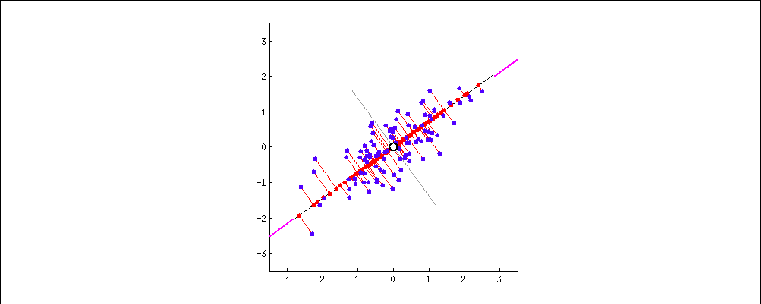
\includegraphics[scale=0.5]{images/PCA_L.png}
		\caption{Prinzipiele Linie}
		\label{PL}
\end{figure}

In der Abbildung \ref{PL} ist die Linie mit der größte Variation und so ist die die erste Prinzipielle Komponente (PK), da sie mit sich die meiste Information trägt. Falls die Variablen dann mit Hilfe dieser PK transformiert werden, wird die meiste Information übertragen. Nachdem die erste Komponente gewählt wird, wird die zweite auf den selben Prinzip gewählt, jedoch wird eine andere Linie gesucht, die dann unabhängig von der erste, meisten eine die Orthogonal zu der Erste liegt. Diese zweite besitzt entsprechend die zweitgrößte Varianz zu den Variablen aus der Datensammlung. Dieser Prozes wiederholt sich bis alle prinzipiellen Komponenten bestimmt sind, oder \emph{p} oft -  genau so oft wie wir Variablen in unsere Kovarianzmatrix haben.

Nun zurück zu den Eigenwerten und -vektoren. Zu Jedem Eigenwert gehört ein Vektor und umgekehrt. Sie Kommen immer in Paare und ihre Anzahl entspricht die dimensionalität der Matrix, wie schon oben erwähnt wurden. Ihre Beziehung in mathematischer Form kann wie folgt dargestellt werden:

\begin{equation}\label{gl1}
	Av = \lambda v,
\end{equation}

wo $\emph{A}$ ist die Matrix, $\emph{v}$ der Eigenvektor und $\lambda$ der zugehörige Eigenwert. Es existiert für eine quadratische Matrix einen Vektor $\emph{v}$ und einen Faktor $\lambda$, sodass bei der Multiplikation der Matrix mit dem Vektor, erhalten wir das gleiche Ergebnis, wie wenn wir den Vektor mit dem Faktor multiplizieren. Es kann die Formel in \ref{gl1} umgeformt werden, um nun die Eigenvektoren und Eigenwerte zu berechnen:

\begin{equation}
	(A - \lambda E).v = 0.
\end{equation}

In der Gleichung enspricht $\emph{E}$ gleich der Einheitsmatrix. Der Eigenvektor ist Lösung der Gleichungssystem. Wir setzte für $\lambda$ den entsprechenden Wert ein und lösen nach v. Jedoch muss der Eigenwert zuerst berechnet werden. Der wird aus der folgenden Formel errechnet:

\begin{equation}
	det(A - \lamda E) = 0
\end{equation}

Wo wir nach den Nullstellen der Determinante suchen. Diese Nullstellen sind die Eingenwerte der Matrix A.

Die Eigenvektoren bestimmen eigentlich die Richtung der Axen mit der meisten Information, oder auch Prinzipielle Komponenten genannt. Die Eingewerte sind die Koeffizienten der Komponente. Je höher der Wert, desto mehr Information wird durch ihre Richtung repräsentiert. Falls die Eigenvektoren nach ihren Eigenwerte absteigend geordnet sind, werden die Ordnung der Prinzipiellen Komponenten bestimmt, sodass die erste Komponente entsprechend diese ist, die den größten Eigenwert besitzt. Als alle Vektoren angeordnet sind, wird einen neuen Vektor aus den zusammengesetzt. Jeder Eigenvektor ist eine Spalte im neuen Vektor. Als nächstes muss die Entscheidung getroffen werden, wie viele prinzipiellen Komponente erhalten werden. Diese Frage hat keine richtige Antwort, in meinem Fall brauche ich nur zwei Komponenten, um die Daten in einem zweidimensionallen Raum darzustellen.


\subsubsection{4. Transformation der Daten}

Im letzten Schritt wird der Prozess abgeschlossen, indem die Ursprungsdaten nach den gefundenen Richtungen ($\emph{Prinzipiellen Komponenten}$), transformiert werden. Die Folgende Formel beschreibt die Operation:

\begin{equation}\label{transPCA}
	T_{L} = V^T_L * Z^T,
\end{equation}  

wo $T_{L}$ die transformierten, $\emph{V}$ enthält die $\emph{L}$ Prinzipiellen Komponenten und $emph{Z}$ beinhaltet den standardisierten Datensatz. Die erhaltene Matrix $\emph{T}$ hat die gewünschte $\emph{L}$ Anzahl an Komponenten. 


QUELLEN:
https://builtin.com/data-science/step-step-explanation-principal-component-analysis

https://royalsocietypublishing.org/doi/10.1098/rsta.2015.0202

https://en.wikipedia.org/wiki/Principal_component_analysis

https://en.wikipedia.org/wiki/Sample_mean_and_covariance

https://www.kaggle.com/jeffd23/visualizing-word-vectors-with-t-sne

https://towardsdatascience.com/visualizing-word-embedding-with-pca-and-t-sne-961a692509f5

https://towardsdatascience.com/visualization-of-word-embedding-vectors-using-gensim-and-pca-8f592a5d3354

https://studyflix.de/mathematik/eigenwert-1635




%\chapter{Weitere Kapitel}

Die Gliederung h�ngt nat�rlich vom Thema und von der L�sungsstrategie ab. Als n�tzliche
Anhaltspunkte k�nnen die Entwicklungsstufen oder - schritte z.B. der Softwareentwicklung betrachtet werden. N�tzliche Gesichtspunkte erh�lt und erkennt man, wenn man sich
\begin{itemize}
  \item in die Rolle des Lesers oder
  \item in die Rolle des Entwicklers, der die Arbeit z.B. fortsetzen, erg�nzen oder pflegen soll,
\end{itemize}
versetzt. In der Regel wird vorausgesetzt, dass die Leser einen fachlichen Hintergrund haben - z.B. Informatik studiert haben. D.h. nur in besonderen, abgesprochenen F�llen schreibt man in popul�rer Sprache, so dass auch Nicht-Fachleute die Ausarbeitung prinzipiell lesen und verstehen k�nnen.

Die �u�ere Gestaltung der Ausarbeitung hinsichtlich Abschnittformate, Abbildungen, mathematische Formeln usw. wird in \hyperref[Stile]{Kapitel~\ref*{Stile}} kurz dargestellt.
%\chapter{LaTeX-Bausteine}\label{Stile}

Der Text wird in bis zu drei Ebenen gegliedert:

\begin{enumerate}
  \item Kapitel ( \verb \chapter{Kapitel} ), \index{Kapitel}
  \item Unterkapitel  ( \verb \section{Abschnitt} ) und
  \item Unterunterkapitel  ( \verb \subsection{Unterabschnitte} ).
\end{enumerate}

\section{Abschnitt}\index{Abschnitt}
Text der Gliederungsebene 2.


\subsection{Unterabschnitt} \index{Unterabschnitt}
Text der Gliederungsebene 3.
Text Text Text Text Text Text Text Text Text Text Text Text Text Text Text
Beispiel f�r Quelltext\index{Quelltext} \\[2 ex]
\noindent
\begin{minipage}{1.0\textwidth} \small
\begin{lstlisting}
	Prozess 1:
	
	Acquire();
		a := 1;
	Release();
	...
	Acquire();
	if(b == 0)
	{					
		c := 3;
		d := a;
	}				
	Release();
\end{lstlisting}
\end{minipage}

\vspace{2cm}
\noindent
\begin{minipage}{1.0\textwidth} \small
\begin{lstlisting}
	Prozess 2:
	
	Acquire();
		b := 1;
	Release();
	...
	Acquire();
	if(a == 0)
	{					
		c := 5;
		d := b;
	}				
	Release();
\end{lstlisting}
\end{minipage}
\vskip 1em

Gr��ere Code-Fragmente sollten im Anhang eingef�gt werden.

\section{Abbildungen und Tabellen}

Abbildung\index{Abbildung} und Tabellen\index{Tabelle} werden zentriert eingef�gt. Grunds�tzlich sollen sie
erst dann erscheinen, nach dem sie im Text angesprochen wurden (siehe Abb. \ref{a1}). Abbildungen und Tabellen (siehe Tabelle \ref{t1}) k�nnen
im (flie�enden) Text (\verb here ), am Seitenanfang (\verb top ), am Seitenende
(\verb bottom ) oder auch gesammelt auf einer nachfolgenden Seite (\verb page )
oder auch ganz am Ende der Ausarbeitung erscheinen. Letzteres sollte man nur
dann w�hlen, wenn die Bilder g�nstig zusammen zu betrachten sind und die
Ausarbeitung nicht zu lang ist ($< 20$ Seiten).

\begin{figure} %[hbtp]
	\centering
		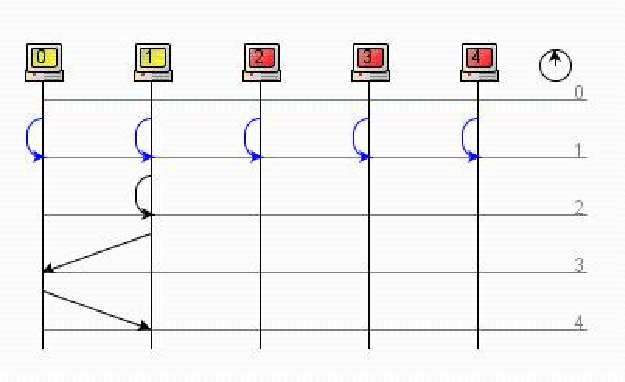
\includegraphics{images/p1ReadSeq.pdf}
	\caption{Bezeichnung der Abbildung}
	\label{a1}
\end{figure}

\begin{table} %[hbtp]
	\centering
		\begin{tabular}{l | l l l l}
		\textbf{Prozesse} & \textbf{Zeit} $\rightarrow$ \\
		\hline
			$P_{1}$ & $W(x)1$ \\
			$P_{2}$ & & $W(x)2$ \\
			$P_{3}$ & & $R(x)2$ & & $R(x)1$\\
			$P_{4}$ & & & $R(x)2$ & $R(x)1$\\
		\end{tabular}
	\caption{Bezeichnung der Tabelle}
	\label{t1}
\end{table}


\section{Mathematische Formel}\index{Formel}
Mathematische Formeln bzw. Formulierungen k�nnen sowohl im
laufenden Text (z.B. $y=x^2$) oder abgesetzt und zentriert im Text
erscheinen. Gleichungen sollten f�r Referenzierungen nummeriert
werden (siehe Formel \ref{gl-1}).
\begin{equation}
\label{gl-1}
e_{i}=\sum _{i=1}^{n}w_{i}x_{i}
\end{equation}

Entscheidungsformel:

\begin{equation}
\psi(t)=\left\{\begin{array}{ccc}
1 &  \qquad 0 <= t < \frac{1}{2} \\
-1 &  \qquad \frac{1}{2} <= t <1 \\
0 & \qquad sonst
\end{array} \right.
\end{equation}


Matrix:\index{Matrix}
\begin{equation}
A = \left(
\begin{array}{llll}
a_{11} & a_{12} & \ldots & a_{1n} \\
a_{21} & a_{22} & \ldots & a_{2n} \\
\vdots & \vdots & \ddots & \vdots \\
a_{n1} & a_{n2} & \ldots & a_{nn} \\
\end{array}
\right)
\end{equation}

Vektor:\index{Vektor} 

\begin{equation}
\overline{a} = \left(
\begin{array}{c}
a_{1}\\
a_{2}\\
\vdots\\
a_{n}\\
\end{array}
\right)
\end{equation}

\section{S�tze, Lemmas und Definitionen}\index{Satz}\index{Lemma}\index{Definition}

S�tze, Lemmas, Definitionen, Beweise,\index{Beweis} Beispiele\index{Beispiel} k�nnen in speziell daf�r vorgesehenen Umgebungen erstellt werden.

\begin{definition}(Optimierungsproblem)

Ein \emph{Optimierungsproblem} $\mathcal{P}$ ist festgelegt durch ein Tupel
$(I_\mathcal{P}, sol_\mathcal{P}, m_\mathcal{P}, goal)$ wobei gilt

\begin{enumerate}
\item $I_\mathcal{P}$ ist die Menge der Instanzen,
\item $sol_\mathcal{P} : I_\mathcal{P} \longmapsto \mathbb{P}(S_\mathcal{P})$ ist eine Funktion, die jeder Instanz $x \in I_\mathcal{P}$ eine Menge zul�ssiger L�sungen zuweist,
\item $m_\mathcal{P} : I_\mathcal{P} \times S_\mathcal{P} \longmapsto \mathbb{N}$ ist eine Funktion, die jedem Paar $(x,y(x))$ mit $x \in I_\mathcal{P}$ und $y(x) \in sol_\mathcal{P}(x)$ eine
Zahl $m_\mathcal{P}(x,y(x)) \in \mathbb{N}$ zuordnet (= Ma� f�r die L�sung $y(x)$ der Instanz $x$), und
\item $goal \in \{min,max\}$.
\end{enumerate}

\end{definition}

\begin{example} MINIMUM TRAVELING SALESMAN (MIN-TSP)
\begin{itemize}
\item $I_{MIN-TSP} =_{def}$ s.o., ebenso $S_{MIN-TSP}$
\item $sol_{MIN-TSP}(m,D) =_{def} S_{MIN-TSP} \cap \mathbb{N}^m$ 
\item $m_{MIN-TSP}((m,D),(c_1, \ldots , c_m)) =_{def} \sum_{i=1}^{m-1} D(c_i, c_{i+1}) + D(c_m,c_1)$ 
\item $goal_{MIN-TSP} =_{def} min$
\end{itemize}
\begin{flushright}
$\qed$
\end{flushright}
\end{example}

\begin{theorem} Sei $\mathcal{P}$ ein \textbf{NP}-hartes Optimierungsproblem.
Wenn $\mathcal{P} \in$ \textbf{PO}, dann ist \textbf{P} = \textbf{NP}.
\end{theorem}

\begin{proof} Um zu zeigen, dass \textbf{P} = \textbf{NP} gilt, gen�gt es
wegen Satz A.30 zu zeigen, dass ein einziges \textbf{NP}-vollst�ndiges
Problem in \textbf{P} liegt. Sei also $\mathcal{P}'$ ein beliebiges \textbf{NP}-vollst�ndiges Problem.

Weil $\mathcal{P}$ nach Voraussetzung \textbf{NP}-hart ist, gilt insbesondere
$\mathcal{P}' \leq_T \mathcal{P}_C$. Sei $R$ der zugeh�rige
Polynomialzeit-Algorithmus dieser Turing-Reduktion.
Weiter ist $\mathcal{P} \in$ \textbf{PO} vorausgesetzt, etwa verm�ge eines
Polynomialzeit-Algorithmus $A$. Aus den beiden
Polynomialzeit-Algorithmen $R$ und $A$ erh�lt man nun
leicht einen effizienten Algorithmus f�r $\mathcal{P}'$: Ersetzt man
in $R$ das Orakel durch $A$, ergibt dies insgesamt eine polynomielle
Laufzeit. 
%\begin{flushright}
$\qed$
% \end{flushright}
\end{proof}

\begin{lemma} Aus \textbf{PO} $=$ \textbf{NPO} folgt \textbf{P} $=$ \textbf{NP}.
\end{lemma}

\begin{proof} Es gen�gt zu zeigen, dass unter der angegeben
Voraussetzung KNAPSACK $\in$ \textbf{P} ist.

Nach Voraussetung ist MAXIMUM KNAPSACK $\in$ \textbf{PO},
d.h. die Berechnung von $m^*(x)$ f�r jede Instanz $x$ ist
in Polynomialzeit m�glich. Um KNAPSACK bei Eingabe
$(x,k)$ zu entscheiden, m�ssen wir nur noch $m^*(x) \geq k$
pr�fen. Ist das der Fall, geben wir $1$, sonst $0$ aus. Dies
bleibt insgesamt ein Polynomialzeit-Algorithmus. 
\begin{flushright}
$\qed$
\end{flushright}
\end{proof}

\section{Fu�noten}

In einer Fu�note k�nnen erg�nzende Informationen\footnote{Informationen die f�r die Arbeit zweitrangig sind, jedoch f�r den Leser interessant sein k�nnten.} angegeben werden. Au�erdem kann eine Fu�note auch Links enthalten. Wird in der Arbeit eine Software (zum Beispiel Java-API\footnote{\url{http://java.sun.com/}}) eingesetzt, so kann die Quelle, die diese Software zur Verf�gung stellt in der Fu�note angegeben werden.

\section{Literaturverweise}\index{Literatur}
Alle benutzte Literatur wird im Literaturverzeichnis angegeben\footnote{Dazu wird ein sogennanter bib-File, literatur.bib verwendet.}. Alle angegebene Literatur sollte mindestens einmal im Text referenziert werden\cite{Coulouris:02}.
%\chapter{Beispiel-Kapitel}

In diesem Kapitel wird beschrieben, warum es unterschiedliche Konsistenzmodelle\index{Konsistenzmodelle} gibt. Au�erdem werden die Unterschiede zwischen strengen Konsistenzmodellen\index{Linearisierbarkeit} (Linearisierbarkeit, sequentielle Konsistenz)\index{sequentiell!Konsistenz} und schwachen Konsistenzmodellen\index{Konsistenz!schwach} (schwache Konsistenz, Freigabekonsistenz)\index{Freigabekonsistenz} erl�utert. Es wird gekl�rt, was Strenge und Kosten (billig, teuer) in Zusammenhang mit Konsistenzmodellen bedeuten.

\section{Warum existieren unterschiedliche Konsistenzmodelle?}

Laut \cite{Malte:97} sind mit der\index{Replikation} Replikation von Daten immer zwei gegens�tzliche Ziele verbunden: die Erh�hung der\index{Verf�gbarkeit} Verf�gbarkeit und die Sicherung der\index{Konsistenz} Konsistenz der Daten. Die Form der Konsistenzsicherung bestimmt dabei, inwiefern das eine Kriterium erf�llt und das andere dementsprechend nicht erf�llt ist (Trade-off zwischen Verf�gbarkeit und der Konsistenz der Daten). Stark konsistente Daten sind stabil, das hei�t, falls mehrere Kopien der Daten existieren, d�rfen keine Abweichungen auftreten. Die Verf�gbarkeit der Daten ist hier jedoch stark eingeschr�nkt. Je schw�cher die Konsistenz wird, desto mehr Abweichungen k�nnen zwischen verschiedenen Kopien einer Datei auftreten, wobei die Konsistenz nur an bestimmten Synchronisationspunkten gew�hrleistet wird. Daf�r steigt aber die Verf�gbarkeit der Daten, weil sie sich leichter replizieren lassen.

Nach \cite{Mosberger:93} kann die Performanzsteigerung der schw�cheren Konsistenzmodelle wegen der Optimierung\index{Optimierung} (Pufferung, Code-Scheduling, Pipelines) 10-40 Prozent betragen. Wenn man bedenkt, dass mit der Nutzung der vorhandenen Synchronisierungsmechanismen schw�chere Konsistenzmodelle den Anforderungen der strengen Konsistenz gen�gen, stellt sich der h�here programmiertechnischer Aufwand bei der Implementierung der schw�cheren Konsistenzmodelle als ihr einziges Manko dar.

In \cite{Cheriton:85} ist beschrieben, wie man sich Formen von DSM vorstellen k�nnte, f�r die ein beachtliches Ma� an\index{Inkonsistenz} Inkonsistenz akzeptabel w�re. Beispielsweise k�nnte DSM verwendet werden, um die Auslastung von Computern in einem Netzwerk zu speichern, so dass Clients f�r die Ausf�hrung ihrer Applikationen die am wenigsten ausgelasteten Computer ausw�hlen k�nnen. Weil die Informationen dieser Art innerhalb k�rzester Zeit ungenau werden k�nnen (und durch die Verwendung der veralteten Daten keine gro�en Nachteile entstehen k�nnen), w�re es vergebliche M�he, sie st�ndig f�r alle Computer im System konsistent zu halten \cite{Coulouris:02}. Die meisten Applikationen stellen jedoch strengere Konsistenzanforderungen.

\section{Klassifizierung eines Konsistenzmodells}

Die zentrale Frage, die f�r die Klassifizierung\index{streng}\index{schwach} (streng oder schwach) eines Konsistenzmodells von Bedeutung ist \cite{Coulouris:02}: wenn ein Lesezugriff auf eine Speicherposition erfolgt, welche Werte von Schreibzugriffen auf diese Position sollen dann dem Lesevorgang bereitgestellt werden? Die Antwort f�r das schw�chste Konsistenzmodell lautet: von jedem Schreibvorgang, der vor dem Lesen erfolgt ist, oder in der "`nahen"' Zukunft, innerhalb des definierten Betrachtungsraums, erfolgten wird. Also irgendein Wert, der vor oder nach dem Lesen geschrieben wurde.

F�r das strengste Konsistenzmodell, Linearisierbarkeit (atomic consistency), stehen alle geschriebenen Werte allen Prozessoren sofort zur Verf�gung: eine Lese-Operation gibt den aktuellsten Wert zur�ck, der geschrieben wurde, bevor das Lesen stattfand. Diese Definition ist aber in zweierlei Hinsicht problematisch. Erstens treten weder Schreib- noch Lese-Operationen zu genau einem Zeitpunkt auf, deshalb ist die Bedeutung von "`aktuellsten"' nicht immer klar. Zweitens ist es nicht immer m�glich, genau festzustellen, ob ein Ereignis vor einem anderen stattgefunden hat, da es Begrenzungen daf�r gibt, wie genau Uhren in einem verteilten System synchronisiert werden k�nnen.

Nachfolgend werden einige Konsistenzmodelle absteigend nach ihrer Strenge vorgestellt. Zuvor m�ssen wir allerdings kl�ren, wie die Lese- und Schreibe-Operationen in dieser Ausarbeitung dargestellt werden.

Sei $x$ eine Speicherposition, dann k�nnen Instanzen dieser Operationen wie folgt ausgedr�ckt werden:
\begin{itemize}
	\item $R(x)a$ - eine Lese-Operation\index{Operation!Lese}, die den Wert $a$ von der Position $x$ liest.
	\item $W(x)b$ - eine Schreib-Operation\index{Operation!Schreib}, die den Wert $b$ an der Position $x$ speichert.
\end{itemize}

\section{Linearisierbarkeit\index{Linearisierbarkeit} (atomic consistency)}

Die Linearisierbarkeit im Zusammenhang mit DSM kann wie folgt definiert werden:
\begin{itemize}
	\item Die verzahnte Operationsabfolge findet so statt: wenn $R(x)a$ in der Folge vorkommt, dann ist die letzte Schreib-Operation, die vor ihr in der verzahnten Abfolge auftritt, $W(x)a$, oder es tritt keine Schreib-Operation vor ihr auf und $a$ ist der Anfangswert von $x$. Das bedeutet, dass eine Variable nur durch eine Schreib-Operation ge�ndert werden kann.
	\item Die Reihenfolge der Operationen in der Verzahnung ist konsistent zu den \underline{Echtzeiten}\index{Echtzeiten}, zu denen die Operationen bei der tats�chlichen Ausf�hrung aufgetreten sind.
\end{itemize}

Die Bedeutung dieser Definition kann an folgendem Beispiel (Tabelle \ref{tab:1}) nachvollzogen werden. Es sei angenommen, dass alle Werte mit $0$ vorinitialisiert sind.

\begin{table}
	\centering
		\begin{tabular}{l | l l l l}
			\textbf{Prozesse} & \textbf{Zeit} $\rightarrow$ & \\
			\hline
			$P_{1}$ & $W(x)1$ & & $W(y)2$ \\
			$P_{2}$ & & $R(x)1$ & & $R(y)2$ \\
		\end{tabular}
	\caption{Linearisierbarkeit ist erf�llt}
	\label{tab:1}
\end{table}

Hier sind beide Bedingungen erf�llt, da die Lese-Operationen den zuletzt geschriebenen Wert zur�ckliefern. Interessanter ist es, zu sehen, wann die Linearisierbarkeit verletzt ist.

\begin{table}
	\centering
		\begin{tabular}{l | l l l l}
		\textbf{Prozesse} & \textbf{Zeit} $\rightarrow$ \\
		\hline
		$P_{1}$ & $W(x)1$ & $W(x)2$ \\
		$P_{2}$ & & & \color{red} $R(x)0$ & \color{black} $R(x)2$ \\
		\end{tabular}
	\caption{Linearisierbarkeit ist verletzt, sequentielle Konsistenz ist erf�llt.}
	\label{tab:2}
\end{table}

In diesem Beispiel (Tabelle \ref{tab:2}) ist die Echtzeit-Anforderung verletzt, da der Prozess $P_{2}$ immer noch den alten Wert liest, obwohl er von Prozess $P_{1}$ bereits ge�ndert wurde. Diese Ausf�hrung w�re aber sequentiell konsistent (siehe kommender Abschnitt), da es eine Verzahnung der Operationen gibt, die diese Werte liefern k�nnte ($R(x)0$, $W(x)1$, $W(x)2$, $R(y)2$). W�rde man beide Lese-Operationen des 2. Prozesses vertauschen, wie in der Tabelle \ref{tab:3} dargestellt, so w�re keine sinnvolle Verzahnung mehr m�glich.

\begin{table}
	\centering
		\begin{tabular}{l | l l l l}
		\textbf{Prozesse} & \textbf{Zeit} $\rightarrow$ \\
		\hline
		$P_{1}$ & $W(x)1$ & $W(x)2$ \\
		$P_{2}$ & & & \color{red} $R(x)2$ &  \color{red} $R(x)0$ \\
			
		\end{tabular}
	\caption{Linearisierbarkeit und sequentielle Konsistenz sind verletzt.}
	\label{tab:3}
\end{table}

In diesem Beispiel sind beide Bedingungen verletzt. Selbst wenn die Echtzeit, zu der die Operationen stattgefunden haben, ignoriert wird, gibt es keine Verzahnung einzelner Operationen, die der Definition entsprechen w�rde.
\chapter{Zusammenfassung und Ausblick}

In diesem Kapitel soll die Arbeit noch einmal kurz zusammengefasst werden. Insbesondere sollen die wesentlichen Ergebnisse Ihrer Arbeit herausgehoben werden. Erfahrungen, die z.B. Benutzer mit der Mensch-Maschine-Schnittstelle gemacht haben oder Ergebnisse von Leistungsmessungen sollen an dieser Stelle pr�sentiert werden. Sie k�nnen in diesem Kapitel auch die Ergebnisse oder das Arbeitsumfeld Ihrer Arbeit kritisch bewerten. W�nschenswerte Erweiterungen sollen als Hinweise auf weiterf�hrende Arbeiten erw�hnt werden.
% ...
%--------------------------------------------------------------------------
\backmatter                        		% Anhang
%-------------------------------------------------------------------------
\bibliographystyle{geralpha}			% Literaturverzeichnis
\bibliography{literatur}     			% BibTeX-File literatur.bib
%--------------------------------------------------------------------------
\printindex 							% Index (optional)
%--------------------------------------------------------------------------
\begin{appendix}						% Anh�nge sind i.d.R. optional
   \chapter{Glossar}

\abbreviation{DisASTer}		{DisASTer (Distributed Algorithms Simulation Terrain), A platform for the Implementation of Distributed Algorithms}
\abbreviation{DSM}			{Distributed Shared Memory}
\abbreviation{AC}			{Linearisierbarkeit (atomic consistency)}
\abbreviation{SC}			{Sequentielle Konsistenz (sequential consistency)}
\abbreviation{WC}			{Schwache Konsistenz (weak consistency)}
\abbreviation{RC}			{Freigabekonsistenz (release consistency)}
			% Glossar   
   \inputencoding{latin1}
\chapter{Erkl�rung der Kandidatin / des Kandidaten}

\begin{description}[$\Box$~]
\item[$\Box$] Die Arbeit habe ich selbstst�ndig verfasst und keine anderen als die angegebenen Quellen- und Hilfsmittel verwendet.\\

\item[$\Box$] Die Arbeit wurde als Gruppenarbeit angefertigt. Meine eigene Leistung ist\\
...\\

Diesen Teil habe ich selbstst�ndig verfasst und keine anderen als die angegebenen Quellen und Hilfsmittel verwendet. \\

\end{description}

\vspace{2cm}

\begin{minipage}[t]{3cm}
\rule{3cm}{0.5pt}
Datum
\end{minipage}
\hfill
\begin{minipage}[t]{9cm}
\rule{9cm}{0.5pt}
Unterschrift der Kandidatin / des Kandidaten
\end{minipage}
   	% Selbstst�ndigkeitserkl�rung
\end{appendix}

\end{document}
